\documentclass[11pt]{article}
\usepackage[a4paper,margin=1in]{geometry}
\usepackage{amsmath,amssymb,amsthm,mathtools}
\usepackage{graphicx}
\usepackage{hyperref}
\usepackage{microtype}

\newtheorem{theorem}{Theorem}
\newtheorem{corollary}{Corollary}
\newcommand{\Rd}{\mathbb R^n}
\newcommand{\E}{\mathcal E}

\title{Multiplicative closure of Levitan and Poisson multipliers}
\author{Run \texttt{fa\_banach\_001}, agent lane 10}
\date{2026-08-12}

\begin{document}
\maketitle

\section*{Source and answer}

Chaouchi, Kosti\'c, and Velinov \cite{source} ask whether, for
$c\in\mathbb C\setminus\{0,1\}$, there can be a bounded continuous
$F:\Rd\to\mathbb C$ which is Levitan $(N,c)$-almost periodic but not
Levitan $(N,c^2)$-almost periodic, or which is uniformly $c$-Poisson stable
but not uniformly $c^2$-Poisson stable.

\begin{center}
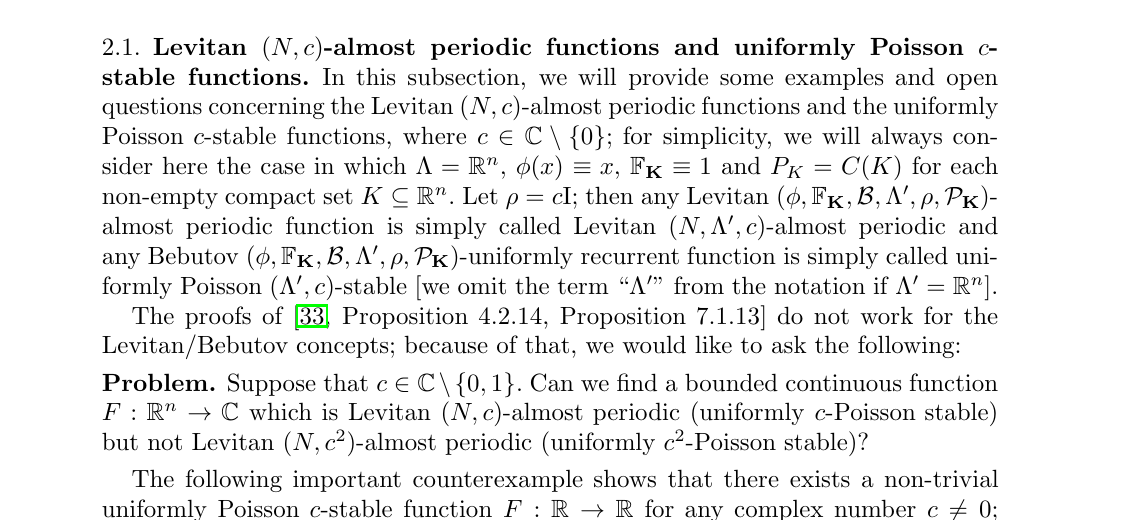
\includegraphics[width=0.96\linewidth]{figures/source_problem.png}
\end{center}

The answer is no in both cases.  More generally, the multiplier classes obey
a multiplicative composition law.  Consequently, membership for $c$
automatically implies membership for every positive integral power $c^m$.
Neither boundedness nor continuity is used in this implication.

\section*{Definitions in the source's specialization}

For a compact set $K\subset\Rd$, a function $F:\Rd\to X$ into a normed
complex vector space, a multiplier $a\in\mathbb C$, and $\epsilon>0$, put
\[
 \E_a(K,\epsilon)
 :=\left\{\tau\in\Rd:
       \sup_{t\in K}\|F(t+\tau)-aF(t)\|\le\epsilon\right\}.
\]
In the specialization used immediately before the source problem,
$F$ is Levitan $(N,a)$-almost periodic precisely when
$\E_a(K,\epsilon)$ is relatively dense in $\Rd$ for every compact $K$ and
every $\epsilon>0$.  It is uniformly $a$-Poisson stable precisely when, for
every compact $K$, there is a sequence $(\tau_j)$ with
$|\tau_j|\to\infty$ and
\[
 \sup_{t\in K}\|F(t+\tau_j)-aF(t)\|\longrightarrow0.
\]
The sequence is allowed to depend on $K$, exactly as in Definition 2.3(ii)
of the source.

\section*{Proof intuition}

Two approximate multiplier-return translations can be performed in
succession.  First move by an $a$-return on $K$; then move by a $b$-return
on the translated compact set.  The composite translation returns $F$ to
$abF$, with the two errors joined by one triangle inequality.  Relative
density survives the fixed first translation.  For Poisson stability, the
second return can be chosen much larger than the first, preventing
cancellation and forcing the composite translations to escape to infinity.

\section*{The composition theorem}

\begin{theorem}[Multiplicative closure]\label{thm:composition}
Let $a,b\in\mathbb C$ and $F:\Rd\to X$.
\begin{enumerate}
\item If $F$ is Levitan $(N,a)$-almost periodic and Levitan
      $(N,b)$-almost periodic, then it is Levitan $(N,ab)$-almost periodic.
\item If $F$ is uniformly $a$-Poisson stable and uniformly $b$-Poisson
      stable, then it is uniformly $ab$-Poisson stable.
\end{enumerate}
\end{theorem}

\begin{proof}
Fix a compact $K\subset\Rd$ and $\epsilon>0$, and set
\[
 \delta:=\frac{\epsilon}{1+|b|}.
\]
For the Levitan assertion, choose any
$\sigma\in\E_a(K,\delta)$.  The translated set $K+\sigma$ is compact, so
$\E_b(K+\sigma,\delta)$ is relatively dense.  If
$\tau\in\E_b(K+\sigma,\delta)$ and $t\in K$, then
\begin{align*}
 \|F(t+\sigma+\tau)-abF(t)\|
 &\le \|F((t+\sigma)+\tau)-bF(t+\sigma)\|\\
 &\quad+|b|\,\|F(t+\sigma)-aF(t)\|\\
 &\le (1+|b|)\delta=\epsilon.
\end{align*}
Therefore
\[
 \sigma+\E_b(K+\sigma,\delta)
 \subseteq \E_{ab}(K,\epsilon).
\]
The set on the left is a translate of a relatively dense set, hence is
relatively dense.  This proves the first assertion.

For the Poisson assertion, choose from $a$-Poisson stability on $K$ a
sequence $(\sigma_j)$ such that
\[
 \sup_{t\in K}\|F(t+\sigma_j)-aF(t)\|
 \le \frac{1}{j(1+|b|)}.
\]
(Passing to a tail or subsequence gives this normalization.)  For the
compact set $K+\sigma_j$, $b$-Poisson stability supplies a sequence of
translations tending to infinity and whose error there tends to zero.
Choose one term $\tau_j$ so far out that
\[
 |\tau_j|>j+|\sigma_j|,
 \qquad
 \sup_{s\in K+\sigma_j}\|F(s+\tau_j)-bF(s)\|
 \le\frac{1}{j(1+|b|)}.
\]
Set $\rho_j=\sigma_j+\tau_j$.  Then
$|\rho_j|\ge |\tau_j|-|\sigma_j|>j$, while the same two-step estimate gives
\[
 \sup_{t\in K}\|F(t+\rho_j)-abF(t)\|\le\frac1j.
\]
Thus $(\rho_j)$ witnesses uniform $ab$-Poisson stability on $K$.
\end{proof}

\begin{corollary}[Power closure and resolution of the problem]
If $F$ is Levitan $(N,c)$-almost periodic, then it is Levitan
$(N,c^m)$-almost periodic for every integer $m\ge1$.  If $F$ is uniformly
$c$-Poisson stable, then it is uniformly $c^m$-Poisson stable for every
integer $m\ge1$.  Hence neither function requested in the source problem
exists.
\end{corollary}

\begin{proof}
The case $m=1$ is the hypothesis.  If the conclusion holds for $m$, apply
Theorem \ref{thm:composition} with $a=c^m$ and $b=c$.  Induction proves the
claim, and $m=2$ answers both alternatives in the problem.
\end{proof}

\section*{Checks, scope, and novelty}

The proof was checked directly against Definition 2.3 and the specialization
in Section 2.1 of the source.  The only structural facts used are that a
translate of a relatively dense subset of $\Rd$ remains relatively dense,
that $K+\sigma$ is compact, and the triangle inequality.  In particular,
the diagonal choice in the Poisson proof is necessary because the source's
recurrence sequence may depend on the compact set.

The theorem applies in all dimensions and, unchanged, to functions with
values in any complex normed space.  It does not require boundedness or
continuity.  It answers exactly the displayed $c$ versus $c^2$ problem; it
does not address the paper's other open questions.

On 2026-08-12, the four cheap run indexes, exact-problem and exact-title
searches, citation searches, and targeted searches for Levitan
$(N,c^2)$ and uniformly $c^2$-Poisson stability found no later claimed
resolution.  This is a bounded novelty check, not an exhaustive survey of
all non-arXiv literature.

\section*{Human review recommendation}

Review as a likely-valid full negative solution.  The highest-value checks
are that the simplified definitions above match the source specialization,
and that the second Poisson translation is chosen on the shifted compact
set $K+\sigma_j$.  Once those points are fixed, both conclusions follow
from the displayed two-step triangle inequality.

\begin{thebibliography}{9}
\bibitem{source}
B.~Chaouchi, M.~Kosti\'c, and D.~Velinov,
\emph{Metrical almost periodicity: Levitan and Bebutov concepts},
arXiv:2209.13576 (2022), especially Definition 2.3 and Section 2.1.
\end{thebibliography}

\end{document}
